\documentclass[10pt,letterpaper]{article}
\usepackage[lmargin=2.2in,rmargin=0.7in,tmargin=1.0in,bmargin=1.0in]{geometry}
\usepackage{notes}
\begin{document}

\begin{center}
\Large\textbf{3.5 - Piecewise Forcing and Convolution}\\
\normalsize (Section 3.2, 3.3)
\end{center}


%%%%%%%%%%%%%%%%%%%%%%%%%%%%%%%%%%%%%%%%%%%%%%%%%%%%%%%%%%%%%%%%%%%%%%%%
\section{First-Order with Piecewise Forcing}

\subsection{Returning to the Harvesting Model}

Last lecture, we introduced a fish farm containing $100$ fish.
After five years, harvesting begins at $30$ fish per year:
\[
p'=0.1p-30H(t-5),\qquad p(0)=100.
\]
The continuous solution is plotted below. We will solve
this IVP in two ways: separately before and after the switch,
then using Laplace transforms.

\begin{figure}[H]
\centering
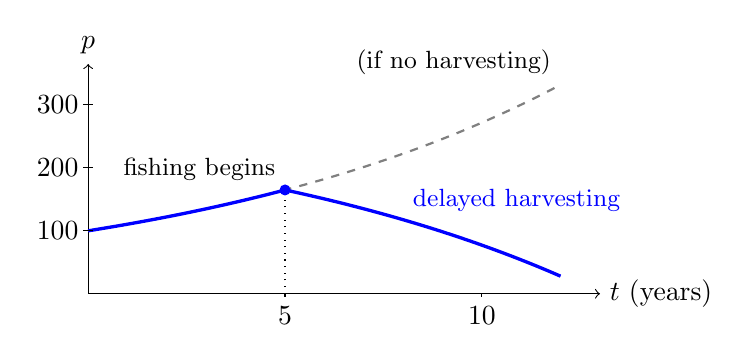
\begin{tikzpicture}[x=0.5cm,y=0.008cm]
    % Axes
    \draw[->] (0,0) -- (13,0)
        node[right] {$t$ (years)};
    \draw[->] (0,0) -- (0,365)
        node[above] {$p$};

    % No harvesting
    \draw[gray,dashed,thick,domain=0:12,samples=150]
        plot (\x,{100*exp(0.1*\x)});

    % Before harvesting
    \draw[blue,very thick,domain=0:5,samples=100]
        plot (\x,{100*exp(0.1*\x)});

    % After harvesting begins
    \draw[blue,very thick,domain=5:12,samples=150]
        plot (\x,{
            300+(100*exp(0.5)-300)*exp(0.1*(\x-5))
        });

    % Switching time
    \draw[dotted] (5,0) -- (5,{100*exp(0.5)});
    \fill[blue] (5,{100*exp(0.5)}) circle (2pt);
    \node[above left] at (5,{100*exp(0.5)})
        {\small fishing begins};

    % Tick labels
    \foreach \t in {5,10}{
        \draw (\t,0) -- (\t,-5);
        \node[below] at (\t,-5) {$\t$};
    }
    \foreach \p in {100,200,300}{
        \draw (-0.12,\p) -- (0.12,\p);
        \node[left] at (0,\p) {$\p$};
    }

    % Curve labels
    \node[above left] at (12,{100*exp(1.2)})
        {\small (if no harvesting)};
    \node[above right,blue] at (8,115)
        {\small delayed harvesting};
\end{tikzpicture}
\end{figure}
%-------------------------------------------------------------
\subsection{Solving in Pieces}

We split the IVP into two sub-problems. Let $p_1(t)$ describe
the population before harvesting begins, and let $p_2(t)$
describe the population afterward. Our goal is to find
both functions and combine them:
\[
p(t)=
\begin{dcases}
p_1(t), & 0\le t<5,\\
p_2(t), & t\ge5.
\end{dcases}
\]
The functions $p_1$ and $p_2$ are solutions to the sub-problems: 
\[
\begin{dcases}
p_1'=0.1 p_1,\\
p_1(0)=100.
\end{dcases} \qquad 
\begin{dcases}
p_2'=0.1 p_2-30,\\
p_2(5)=k.
\end{dcases}
\]
There are two key differences in the sub-problems. First, the DEs are different because of the Heaviside term $f=-30H(t-5)$. Second, the initial conditions are different. The condition $p_1(0)=100$ is a given condition. The IC for $p_2$ begins at $t=5$ and the value $k$ must be determined after solving for $p_1$. The value for $k$ is 
$$
    k = p_1(5).
$$
This condition ensures that piecewise function $p(t)$ is continuous at $t=5$.

\begin{example}[1]{
Solve the IVP in pieces using the method of
undetermined coefficients:
\[
p'=0.1p-30H(t-5),\qquad p(0)=100.
\]
}

\paragraph{Step 1. Solve for $p_1$.}
Before harvesting,
\[
p_1'=0.1p_1,\qquad p_1(0)=100,
\]
so
\[
p_1(t)=100e^{0.1t},
\qquad p_1(5)=100e^{1/2}.
\]

\paragraph{Step 2. Solve for $p_2$.}
The second sub-problem is
\[
p_2'-0.1p_2=-30,\qquad p_2(5)=100e^{1/2}.
\]
The homogeneous solution is $Ce^{0.1t}$. Trying a constant
particular solution $p_p(t)=A$ gives $-0.1A=-30$, so $A=300$.
Thus, the general solution is
\[
p_2(t)=Ce^{0.1t}+300.
\]
Applying the initial condition,
\[
p_2(5)=Ce^{1/2}+300\equiv100e^{1/2}
\implies C=100-300e^{-1/2}.
\]
Therefore,
\[
p_2(t)=100e^{0.1t}
+300\bigl(1-e^{0.1(t-5)}\bigr).
\]

\paragraph{Step 3. Combine $p_1$ and $p_2$.}
Use each solution on its corresponding interval:
\[
\boxed{
p(t)=
\begin{dcases}
100e^{0.1t}, & 0\le t<5,\\
100e^{0.1t}+300\bigl(1-e^{0.1(t-5)}\bigr),
& t\ge5.
\end{dcases}
}
\]
\end{example}


%-------------------------------------------------------------
\subsection{Solving with Laplace Transforms}

Laplace transforms let us solve the IVP without splitting
it into sub-problems. We obtain an answer in Heaviside
notation, then rewrite it piecewise.

\begin{example}[2]{
Solve the same IVP using Laplace transforms:
\[
p'=0.1p-30H(t-5),\qquad p(0)=100.
\]
Write the answer using Heaviside notation and in piecewise form.
}

\paragraph{Step 1. Transform and solve for $P(s)$.}
Let $P(s)=\mathcal L[p(t)]$. Taking transforms gives
\[
sP(s)-100=0.1P(s)-30\frac{e^{-5s}}{s}.
\]
Solving for $P(s)$,
\[
P(s)=\frac{100}{s-0.1}
-30e^{-5s}
\underbrace{\frac{1}{s(s-0.1)}}_{G(s)}.
\]

\paragraph{Step 2. Find the inverse of the rational part.}
Ignore the $-30e^{-5s}$ factor for the time being, and focus on the rational factor $G(s)$. Using partial fractions,
\[
G(s)=-\frac{10}{s}+\frac{10}{s-0.1},
\]
so the inverse transform is
\[
g(t)=\mathcal L^{-1}[G(s)]
=10\bigl(e^{0.1t}-1\bigr).
\]

\paragraph{Step 3. Find the full inverse.}
The switching property gives
\[
p(t)=100e^{0.1t}-30H(t-5)g(t-5).
\]
Substituting $g(t-5)$,
\[
\boxed{
p(t)=100e^{0.1t}
+300H(t-5)\bigl(1-e^{0.1(t-5)}\bigr).
}
\]
Setting $H(t-5)=0$ before the switch and $1$ afterward,
\[
\boxed{
p(t)=
\begin{dcases}
100e^{0.1t}, & 0\le t<5,\\
100e^{0.1t}+300\bigl(1-e^{0.1(t-5)}\bigr),
& t\ge5.
\end{dcases}
}
\]
This agrees with the solution obtained in pieces.
\end{example}



%%%%%%%%%%%%%%%%%%%%%%%%%%%%%%%%%%%%%%%%%%%%%%%%%%%%%%%%%%%%%%%%%%%%%%%%
\section{Second-Order with Piecewise Forcing}

\subsection{A Delayed Forcing Term}
The Laplace transform method also applies to second-order
equations with piecewise forcing. Consider the problem
\[
x''-x=g(t),
\qquad x(0)=1,\quad x'(0)=0,
\]
where
\[
g(t)=
\begin{dcases}
0, & 0\le t<2,\\
2\cos(t-2), & t\ge2.
\end{dcases}
\]
The first step to solving this equation is to rewrite $f(t)$ using the Heaviside function:
\[
g(t)=2\cos(t-2)H(t-2).
\]
We will need to transform the forcing term as well
\[
\mathcal L[g(t)]
=e^{-as}F(s)
=e^{-2s}\frac{2s}{s^2+1}.
\]


%-------------------------------------------------------------
\subsection{Solving with Laplace Transforms}
Follow the 3 steps to solve IVPs involving piecewise functions
\begin{enumerate}
    \item Transform the entire DE and solve for $X(s)$.
    \item Invert the rational part. 
    \item Find the full inverse.
\end{enumerate}
If asked, you should be able to rewrite the solution in piecewise form.

\begin{example}[3]{
Solve the IVP using Laplace transforms:
\[
x''-x=
\begin{dcases}
0, & 0\le t<2,\\
2\cos(t-2), & t\ge2,
\end{dcases}
\qquad x(0)=1,\quad x'(0)=0.
\]
Write the solution using Heaviside notation and in
piecewise form.
}

\paragraph{Step 1. Transform the entire DE and solve for $X$.}
\begin{align*}
   \mathcal{L}\left[  x''-x \right] &= \mathcal{L}\left[2\cos(t-2)H(t-2)\right] \\
s^2X(s)-sx(0)-x'(0)-X(s) &=e^{-2s}\frac{2s}{s^2+1}\\
s^2X(s)-s-X(s)&=e^{-2s}\frac{2s}{s^2+1}\\
(s^2-1)X(s)&=s+e^{-2s}\frac{2s}{s^2+1}\\
X(s)&=
\underbrace{\frac{s}{s^2-1}}_{X_1(s)}
+
e^{-2s}
\underbrace{\frac{2s}{(s^2-1)(s^2+1)}}_{X_2(s)}.
\end{align*}
Ignore $e^{-2s}$ for now, and focus on $X_1$ and $X_2$.

\paragraph{Step 2. Invert the rational part.}
I'll leave it as an exercise for you to verify the following partial fraction decomposition
\[
X_1(s)=\frac{1}{2(s-1)}+\frac{1}{2(s+1)},
\]
and so
\[
X_2(s)=\frac{s}{s^2-1}-\frac{s}{s^2+1}
=\frac{1}{2(s-1)}+\frac{1}{2(s+1)}
-\frac{s}{s^2+1}.
\]
Therefore, the base inverse transforms are 
\[
x_1(t)=\mathcal L^{-1}[X_1(s)]
=\frac12e^t+\frac12e^{-t},
\]
\[
x_2(t)=\mathcal L^{-1}[X_2(s)]
=\frac12e^t+\frac12e^{-t}-\cos t.
\]
\paragraph{Step 3. Find the full inverse.}
At this point, bring $e^{-2s}$ back into the picture. We need to utilize the switch property to find the full inverse:
\begin{align*}
    x(t)&=\mathcal{L}^{-1}\left[ X_1(s) +e^{-2s}X_2(s)\right]\\
        &=x_1(t) + H(t-2)x_2(t-2)\\
        &=\boxed{
        \frac12e^t+\frac12e^{-t}+H(t-2)\left(\frac12e^{(t-2)}+\frac12e^{-(t-2)}-\cos (t-2)\right)}
\end{align*}

% \paragraph{Step 4. Write the answer in piecewise form.}
% Before $t=2$, the Heaviside term is zero.
% Afterward, it adds $g(t-2)$:
% \[
% \boxed{
% x(t)=
% \begin{dcases}
% h(t), & 0\le t<2,\\
% h(t)+g(t-2), & t\ge2.
% \end{dcases}
% }
% \]
% Here, $h(t)$ and $g(t)$ are the functions defined above.
\end{example}

%-------------------------------------------------------------

\subsection{Writing Solutions Compactly}

The \textbf{hyperbolic functions}
\[
\cosh t=\frac{e^t+e^{-t}}{2},
\qquad
\sinh t=\frac{e^t-e^{-t}}{2}
\]
provide convenient shorthand for pairs of exponentials.
For example, when $k>0$,
\[
x''-k^2x=0
\quad\implies\quad
x(t)=c_1\cosh(kt)+c_2\sinh(kt).
\]
Using this notation, the solution to Example 3 becomes
\[
x(t)=\cosh t
+H(t-2)\bigl[\cosh(t-2)-\cos(t-2)\bigr].
\]

More generally, we can name repeated expressions ourselves.
Define
\[
h(t)=\cosh t,
\qquad
g(t)=\cosh t-\cos t.
\]
Then both the Heaviside and piecewise forms are compact:
\[
\boxed{
x(t)=h(t)+H(t-2)g(t-2)
=
\begin{dcases}
h(t), & 0\le t<2,\\
h(t)+g(t-2), & t\ge2.
\end{dcases}
}
\]
Naming functions is a useful way to simplify long answers,
provided those functions are explicitly defined.
%%%%%%%%%%%%%%%%%%%%%%%%%%%%%%%%%%%%%%%%%%%%%%%%%%%%%%%%%%%%%%%%%%%%%%%%
\section{Convolution}

\subsection{Inverting a Product}

So far, we have used partial fractions to rewrite a
transform as a sum of familiar terms. For example,
\[
X(s)=\frac{1}{s(s^2+4)}
\]
can be decomposed and inverted term by term. But this expression is also a product 
\[
X(s)=
\underbrace{\frac1s}_{F(s)}
\underbrace{\frac1{s^2+4}}_{G(s)}.
\]
We know the inverse transform of each factor.
Can we combine them to find the inverse of the product?

Simply multiplying the inverse transforms does not work:
\[
\mathcal L^{-1}[F(s)G(s)]\ne f(t)g(t)
\quad\text{in general}.
\]
Instead, we need a new operation called
\textbf{convolution}.

%-------------------------------------------------------------
\subsection{The Convolution Integral}

The \textbf{convolution} of two functions $f$ and $g$
is defined by
\[
\boxed{
(f*g)(t)=\int_0^t f(t-\tau)g(\tau)\,d\tau.
}
\]
The symbol $*$ denotes convolution, not ordinary
multiplication. Inside the integral, $t$ is treated as a constant
and $\tau$ is the variable of integration.
After integrating and evaluating the endpoints,
the result is a function of $t$.

Convolution is commutative:
\[
f*g=g*f.
\]
Thus, we may also write
\[
(f*g)(t)=\int_0^t f(t-\tau)g(\tau)\,d\tau=\int_0^t f(\tau)g(t-\tau)\,d\tau.
\]
Choose whichever form makes the integration easier.

%-------------------------------------------------------------
\subsection{The Convolution Formula}

If $\mathcal L[f(t)]=F(s)$ and
$\mathcal L[g(t)]=G(s)$, then, wherever the transforms
converge absolutely,
\[
\boxed{\mathcal L[(f*g)(t)]=F(s)G(s).}
\]
This formula is more commonly used in reverse 
\[
\boxed{
\mathcal L^{-1}[F(s)G(s)]
=\int_0^t f(t-\tau)g(\tau)\,d\tau.
}
\]
To use this formula:
\begin{enumerate}
    \item Split the transform into two familiar factors.
    \item Find their inverse transforms.
    \item Form the convolution integral and evaluate it.
\end{enumerate}

%-------------------------------------------------------------
\begin{example}[4]{
Use convolution to find
\[
\mathcal L^{-1}\left[\frac{1}{s(s^2+4)}\right].
\]
Do not leave your answer in terms of integrals.
}

\paragraph{Step 1. Identify the two factors.}
Write
\[
\frac{1}{s(s^2+4)}
=
\underbrace{\frac1s}_{F(s)}
\underbrace{\frac1{s^2+4}}_{G(s)}.
\]

\paragraph{Step 2. Find the inverse transforms.}
From the transform table,
\[
f(t)=1,
\qquad
g(t)=\frac12\sin2t.
\]

\paragraph{Step 3. Evaluate the convolution integral.}
Using $f(t-\tau)=1$ and
$g(\tau)=\frac12\sin2\tau$,
\begin{align*}
x(t)
&=\int_0^t f(t-\tau)g(\tau)\,d\tau\\
&=\frac12\int_0^t\sin2\tau\,d\tau\\
&=\left[-\frac14\cos2\tau\right]_0^t=\boxed{\frac14(1-\cos2t).}
\end{align*}
\end{example}

%-------------------------------------------------------------
\subsection{Forcing beyond Undetermined Coefficients}

The method of undetermined coefficients works for polynomials,
exponentials, sines, cosines, and their sums and products.
But what if the forcing is $e^{-t^2}$?

Repeated differentiation produces polynomials of increasing
degree multiplied by $e^{-t^2}$, so the usual finite trial
form does not work. Convolution lets us write a solution
without choosing a trial function or even finding the
forcing's Laplace transform explicitly.

\begin{example}[5]{
Solve the IVP
\[
x''+9x=e^{-t^2},\qquad x(0)=1,\quad x'(0)=0.
\]
You may leave the answer as a convolution integral.
}

\paragraph{Step 1. Transform the DE.}
Let $X(s)=\mathcal L[x(t)]$ and denote the transform
of the forcing by
\[
F(s)=\mathcal L[e^{-t^2}].
\]
We do not need an explicit formula for $F(s)$.
Taking transforms and using the initial conditions gives
\[
s^2X(s)-s+9X(s)=F(s).
\]

\paragraph{Step 2. Solve for $X(s)$.}
\[
X(s)=\frac{s}{s^2+9}
+\underbrace{\frac{1}{s^2+9}}_{G(s)}F(s).
\]

\paragraph{Step 3. Invert using convolution.}
The first term has inverse $\cos3t$. For the product,
we know both base functions:
\[
g(t)=\mathcal L^{-1}[G(s)]=\frac13\sin3t,
\qquad
f(t)=e^{-t^2}.
\]
By the convolution theorem,
\[
\mathcal L^{-1}[G(s)F(s)]
=\int_0^t g(t-\tau)f(\tau)\,d\tau.
\]
Therefore,
\[
\boxed{
x(t)=\cos3t+
\frac13\int_0^t
\sin\bigl(3(t-\tau)\bigr)e^{-\tau^2}\,d\tau.
}
\]
This is an exact solution. The integral does not need an elementary antiderivative; it can also be evaluated numerically to calculate or plot $x(t)$.

\end{example}



\end{document}